\section{Introduction}
% 20250224: what is KG?
Knowledge Graphs (KGs) store enormous facts in the form of structured triples, i.e., \texttt{<subject, relation, object>}. Many real-world tasks, such as recommendation systems and question answering, have been brought about prosperity with the ability of commonsense understanding and reasoning of KGs~\cite{jiSurveyKnowledgeGraphs2022}.
% 20250224: What's the meaning of KGQA
Among them, Knowledge Graph Question Answering (KGQA) is a task that aims to answer natural language questions based on KGs~\cite{dong2015KGQA}. It has garnered significant attention from academia and industry due to its crucial role in various intelligent applications such as the Google search engine and Apple Siri~\cite{zhouCommonsenseKnowledgeAware2018}.

% % 20250224: what is TKG
% Previous knowledge graph research mostly focuses on static facts that have not changed with time. However, temporal information is very important because structured knowledge is only held within a specific period. To solve this problem, recent research has begun to take temporal information into KGs, which are termed Temporal Knowledge Graphs (TKGs). 

Previous knowledge graph research has predominantly focused on static facts that remain unchanged over time. However, temporal information is crucial, as structured knowledge is often valid only within specific periods. To address this limitation, Temporal Knowledge Graphs (TKGs) have been introduced, incorporating timestamps to represent the temporal dynamics of facts. As illustrated in Figure~\ref{fig:TKGQA-task}, the TKG associates each fact with a specific time point between 1997 and 2001 to denote when \textit{Harry Potter and the Philosopher’s Stone} received various awards. This temporal representation enables TKGs to capture the evolving nature of real-world events, facilitating more accurate reasoning and retrieval of time-sensitive information.

Based on TKG, Temporal Knowledge Graph Question Answering (TKGQA) aims to answer questions that involve temporal constraints or require timestamped answers, referred to as temporal questions in this paper. As illustrated in Figure~\ref{fig:TKGQA-task}, the example question contains the temporal constraint ``last'', which identifies the most recent event in a time sequence. To tackle TKGQA, models must capture the nuances of constraint and the chronological order of events, making it an increasingly prominent challenge in KGQA. However, TKGQA still faces two key challenges: 

\begin{figure}
    \centering
    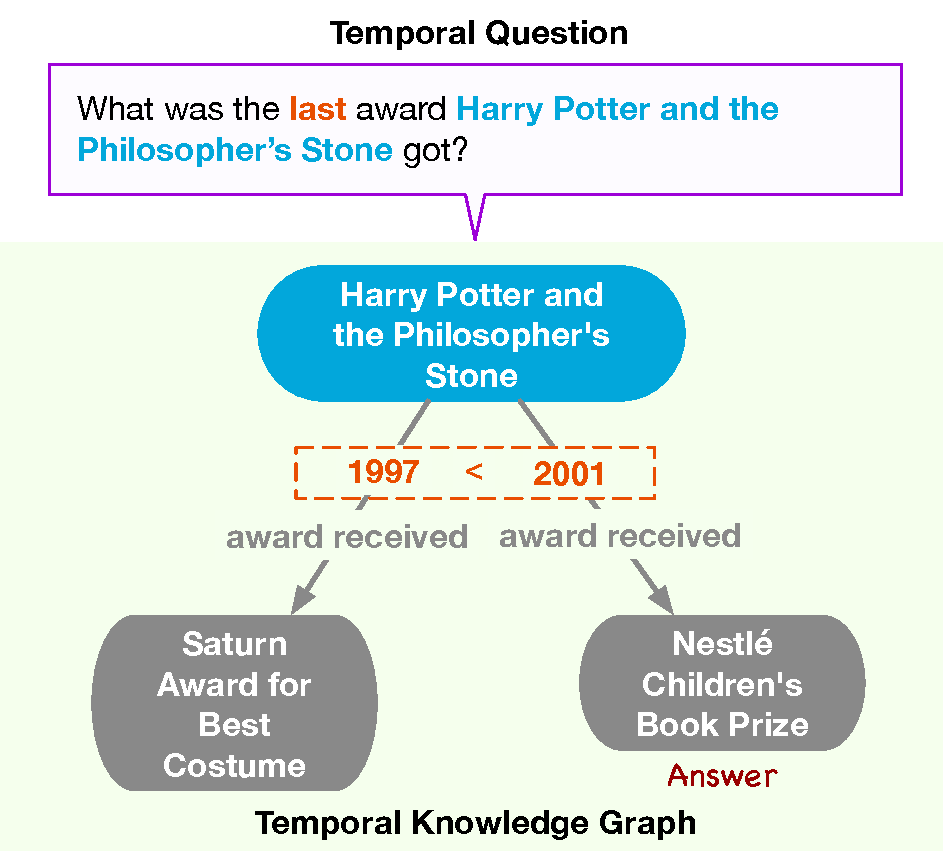
\includegraphics[width=\linewidth]{figures/intro-task.pdf}
    \caption{Given a temporal question (purple box), the TKGQA task aims to derive the answer from the underlying TKG (green box).}
    \label{fig:TKGQA-task}
\end{figure}

% Existing KBQA methods, even those capable of handling complex questions, still perform poorly on temporal questions~\cite{jiaTEQUILATemporalQuestion2018, sun2019pullnet, pramanik2021uniqorn,AQQU,QUINT}.
% reported mean F1 scores of 27.2 and 30.0 for AQQU~\cite{AQQU} and QUINT~\cite{QUINT} on TempQuestions. The Neural-Symbolic Reasoning system PullNet~\cite{sun2019pullnet} achieved an F1 score of 54.2 on TimeQuestions, while Uniqorn~\cite{pramanik2021uniqorn}, which uses group Steiner trees, scored 33.1.
% To address this, researchers introduced temporal knowledge graphs (TKGs) that incorporate timestamps into knowledge triples, exemplified by \texttt{<Zhang Weili, win, UFC's strawweight championship, 2024>}~\cite{TKGfirst}.
% These results underscore the complexity of TKGQA tasks. It is particularly challenging for two primary reasons:
% (1) KBQA systems struggle to identify and stress temporal-related information in questions, such as terms like ``before,'' ``2023,'' or ``WWII.'' Even prepositions like ``on'' can affect the answer. (2) Reasoning about time points and intervals is complex and not adequately addressed by current KBQA systems.
% \paragraph{\textbf{Temporal Knowledge Graph Question Answering.}} 
% Some Temporal Knowledge Graph Question Answering (TKGQA) methods are proposed to overcome this barrier. Temporal knowledge graphs (TKGs) incorporate timestamps into knowledge triples, such as \texttt{<Weili Zhang, win, UFC's strawweight championship, 2024>}~\cite{TKGfirst}. 
% TKGQA aims to answer questions containing temporal constraints or requiring timestamp answers based on TKG~\cite{jiaTEQUILATemporalQuestion2018}. 
% This task has garnered significant research interest, leading to various datasets 


(1) \textbf{Inconsistency in the classification of temporal questions.} 
The existing research has not yet formed a unified framework for the type classification criteria of temporal questions. First, individual datasets often mix different classification criteria within a single framework. For example, as shown in Table \ref{tab:dataset}, CronQuestions applies the category \textit{SimpleTime} based on both the answer type and question complexity. At the same time, it also includes \textit{Before/After}, which is determined by content features within the same classification system. This cross-dimensional categorization leads to systematic ambiguity and inconsistency. Secondly, the Venn diagram of TempQuestions and CronQuestions shows that their classification systems have asymmetric overlaps, indicating a lack of logical compatibility between the existing classification systems.

% Accurately classifying temporal questions is essential for effective model design. The classification system determines the question type, which is usually provided as part of the model input~\cite{jia2024faithful,jiaComplexTemporalQuestion2021} or identified by the model itself~\cite{chenTemporalKnowledgeQuestion2024,dingSemanticFrameworkBased2023,shangImprovingTimeSensitivity2022}, influencing various aspects of the model architecture. For example, different scoring functions are required for distinct answer types~\cite{shangImprovingTimeSensitivity2022,chenTemporalKnowledgeGraph2022,qianTimeR4TimeawareRetrievalAugmented2024}, and specific processing modules are necessary for implicit questions~\cite{jiaFaithfulTemporalQuestion2024,chenTemporalKnowledgeGraph2022,duSemanticenhancedReasoningQuestion2024}. If the classification is incorrect or vague, the model may apply inappropriate techniques, leading to inaccurate answers and reduced performance.
Inconsistent classification of temporal questions can lead to several issues in model development and evaluation. If different works adopt conflicting classification schemes, it becomes difficult to compare methods fairly, hindering progress in the field.  This inconsistency can also lead to inefficiencies in model design—some models may apply inappropriate reasoning strategies, while others may lack necessary processing modules for certain question types. Consequently, the field urgently needs a well-defined and consistent classification framework for temporal questions.

\IEEEpubidadjcol

\begin{table}[htbp] 
    \caption{Question types and their Venn Diagram of TKGQA datasets.\label{tab:dataset}}
    \centering
    \begin{threeparttable}
    \resizebox{0.9\columnwidth}{!}{%
    \begin{tabular}{ccc}
    \toprule
        \textbf{Dataset} & \textbf{\makecell{Question\\Types}} & \textbf{Venn Diagram} \\ \midrule
        \makecell[c]{Temp\\Questions} & \makecell[c]{Explicit\\Implicit\\Ordinal\\Temp.Answer} & \makecell{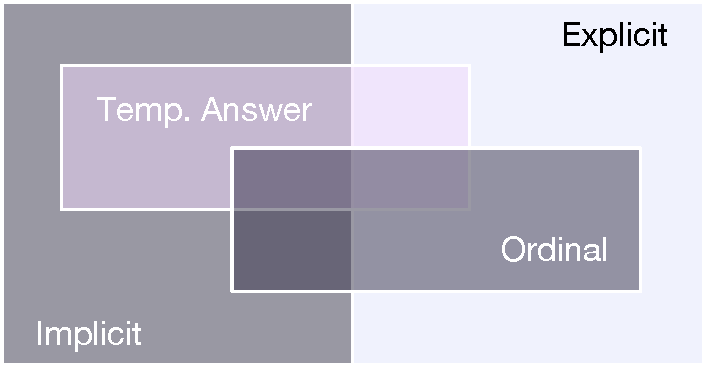
\includegraphics[width=0.3\textwidth]{figures/QuestionTypes-TempQuestions.pdf}}\\ \midrule
        \makecell{Cron\\Questions} & \makecell{SimpleTime\\SimpleEntity\\Before/After\\First/Last\\TimeJoin} & \makecell{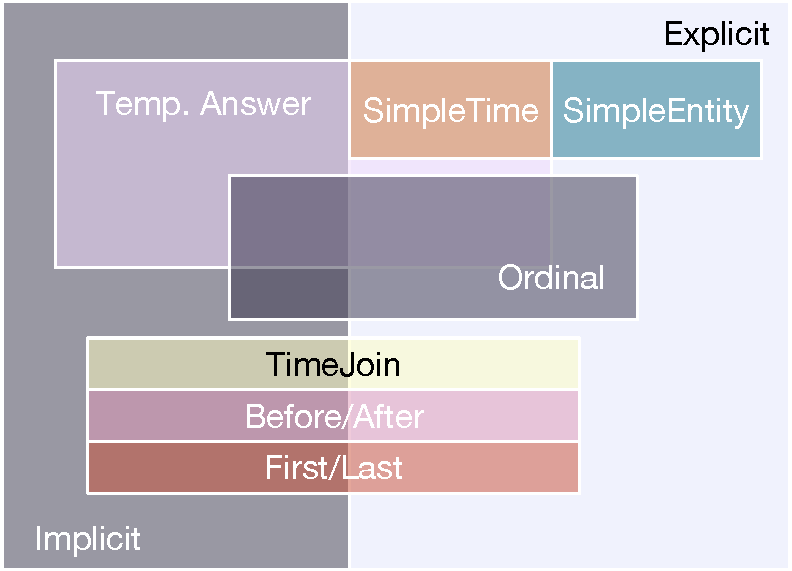
\includegraphics[width=0.3\textwidth]{figures/QuestionTypes-CronQuestions.pdf}}\\ \midrule
        \makecell{MultiTQ} & \makecell{Equal\\Before/After\\First/Last\\Equal Multi\\Before Last\\After First} & \makecell{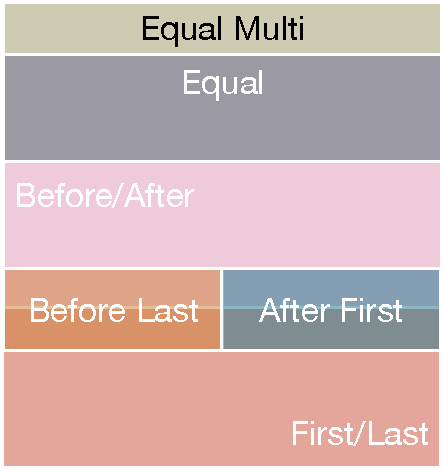
\includegraphics[width=0.2\textwidth]{figures/QuestionTypes-MultiTQ.pdf}} \\ 
    \bottomrule
    \end{tabular}}
    \end{threeparttable}
\end{table}

(2) \textbf{Lack of systematic categorization of existing methods.}
 Existing surveys primarily focus on KGQA methods for static factual questions, adopting a two-tiered classification: \textbf{semantic parsing-based methods} that convert questions into formal logical queries (e.g., SPARQL), and \textbf{information retrieval-based methods} that match questions to answers via scoring mechanisms~\cite{fuSurveyComplexQuestion2020a,lanSurveyComplexKnowledge2021}. This framework effectively captures core technical distinctions in conventional KGQA where temporal dynamics are absent.

However, these classifications prove inadequate for TKGQA due to three inherent reasons:
\begin{inparaenum}[(i)]
\item The commonly used quadruple structure \texttt{<subject, relation, object, timestamp>} in TKGQA demands specialized temporal grounding mechanisms beyond static triple processing;
\item Diverse temporal question types require dedicated reasoning architectures;
\item The emergence of LLMs introduces new methodological paradigms that transcend traditional categorization.
\end{inparaenum}
Current surveys neither provide granular taxonomies for temporal-specific reasoning processes nor systematically analyze how LLM capabilities can be operated in temporal contexts~\cite{guKnowledgeBaseQuestion2022a}. This gap obstructs the mapping between question types and technical solutions, thereby limiting the ability to select and refine methods in a targeted manner.


To address the above challenges, this paper provides a thorough survey from two perspectives: a taxonomy of temporal questions and a dedicated categorization for TKGQA methods. Our main contributions can be summarized as follows:
\begin{itemize}
    \item We first establish a unified taxonomy that encompasses existing temporal question types and definitions, providing a standardized reference that could be widely adopted and further extended.
    
    \item We systematically categorize existing methods into semantic parsing-based, TKG embedding-based, and LLM-based. Furthermore, we explicate key procedures and techniques especially demanded by various temporal questions. This refined reclassification not only better aligns with the technical principles of TKGQA but also acknowledges emerging trends, such as LLMs’ potential to augment temporal reasoning. 
    
    \item We identify the temporal question types that each method can solve and summarize them in a table. This helps analyze the focus of existing methods and highlight question types that lack attention. Based on this review, we also explore future research directions.

    \item To the best of our knowledge, this is the first comprehensive survey on the TKGQA task. By serving as a comprehensive reference for TKGQA, this work aims to stimulate further research and foster innovation in the field. 
\end{itemize}

The rest of this survey is organized as follows. In §\ref{sec-pre}, we provide detailed definitions of TKGQA and relevant concepts. In §\ref{sec-question}, we classify temporal questions across all datasets based on 
question content (§\ref{question type}), answer type (§\ref{answertype}), and complexity (§\ref{complexity}).
In §\ref{sec-method}, we introduce the three main categories of TKGQA methods; in §\ref{sec-sp}, we detail semantic parsing-based methods, while in §\ref{sec-tkge}, we elaborate on TKG embedding-based methods; furthermore, we dive into LLM-based methods in §\ref{sec-llm}; in §\ref{taskcoverage}, we align each method with the specific types of questions it is designed to solve, providing a detailed summary table. We also introduce the evaluation metrics for TKGQA tasks (§\ref{sec-metrics}) and present a leaderboard illustrating the latest research progress (§\ref{leaderboard}).
In §\ref{future}, we explore new frontiers, summarizing their challenges and highlighting opportunities for further research. We conclude this survey in §\ref{conclusion}. Furthermore, in Appendix \ref{sec-appendix}, we provide a detailed description of the existing TKGQA datasets (§\ref{sec-datasets}), including their underlying temporal knowledge graphs. 

% The rest of this article is organized as follows. 
% \begin{itemize}
%     \item In §\ref{sec-pre}, we define in detail the relevant concepts of TKGQA and this task. To the best of our knowledge, this is the first comprehensive survey on the TKGQA task.
%     \item  In §\ref{sec-question}, we classify temporal questions across all datasets based on multiple aspects and analyze their interdependencies (§\ref{question type}); we also consider the complexity dimension of traditional knowledge-based questions in our classification (§\ref{complexity}).
%     \item In §\ref{sec-method}, we briefly introduce the two approaches to TKGQA methods. In §\ref{sec-sp}, we introduce Semantic Parsing-based Methods detailedly; in §\ref{sec-tkge}, we introduce TKG Embedding-based Methods. 
%     \item In §\ref{conclusion}. we conclude this survey. In §\ref{future}, we explore new frontiers, summarize their challenges, and highlight opportunities for further research.
%     \item We align temporal question types with their capable methods, providing a detailed table and a leaderboard to show the latest research progress in Appendix \ref{sec-appendix}.
% \end{itemize}
% \begin{enumerate}
% \item \textbf{\textit{First survey:}} To the best of our knowledge, this is the first comprehensive survey on the TKGQA task.
% \item \textbf{\textit{New taxonomy:}} We systematically classify temporal question types across all datasets and analyze their interdependencies (see Fig.~\ref{fig:pdfimage}).
% \item \textbf{\textit{Abundant resources:}} We align temporal question types with their capable methods, providing a detailed table in Appendix~\ref{sec-appendix}. We also provide a leaderboard to show the latest research progress.
% \item \textbf{\textit{New Frontiers:}} We summarize relevant TKGQA work and identify future research directions.
% \end{enumerate}
% \paragraph{Related work}